\documentclass[a4paper,12pt]{article}

  \usepackage[utf8]{inputenc}
  \usepackage[T1]{fontenc}
  \usepackage{polski}
  \usepackage{lmodern}
  \usepackage[protrusion=true,expansion=true]{microtype}

  \usepackage{amssymb}
  \usepackage{a4wide}
  \usepackage{amsmath}
  \usepackage{enumerate}
  \usepackage{fancyhdr}
  \usepackage{anysize}
  \usepackage{array}
  \usepackage{multicol}
  \usepackage{verbatim}
  \usepackage{setspace}
  \usepackage{shadow}

%\usepackage{showframe}

  \usepackage{tikz}
  \usepackage{tkz-fct}
  \usepackage{tkz-euclide}
  \usepackage{tkz-base}
  \usetikzlibrary{datavisualization}
  \usetikzlibrary{calc}
  \usetikzlibrary{arrows}
  \usetikzlibrary{automata}
  \usetikzlibrary{backgrounds}
  \usetikzlibrary{decorations}
  \usetikzlibrary {intersections}

  \usepackage{logicpuzzle}


\pagestyle{fancyplain}

\lhead[ \fancyplain { } {\footnotesize\thepage} ]
      { \fancyplain { } {                     } }
\rhead[ \fancyplain { } {                     } ]
      { \fancyplain { } {\footnotesize\thepage} }
\chead[ \fancyplain { } {\footnotesize\leftmark  } ]
      { \fancyplain { } {\footnotesize\leftmark  } }
\cfoot[ ]{ }

%%%%%%%%%%%%%%%%%%%%%%%%%%%%%%%%%%%%%%%%%%%%%%%%%%%%%%%%%%%%%%%%%%%%%%%%%%%%%%%%%%%%%%%%%%%%%%%%%%%%%%%%%%%%%%%%%%%%%%
\newcommand{\znacznik}
{
 \marginpar[\hfill$\boxed{\boldsymbol{!\Rightarrow}}$]
                      {
                       $\boxed{\boldsymbol{!\Leftarrow}}$
                      }
}
%
\newcommand{\itemgw}                           % kolejna pozycja w srodowiku enumerate
      {                                        % na poziomie 1, opatrzona  gwiazdka
       \item[\addtocounter{enumi}{1}\bf\theenumi.\!\!\rlap{*}\;]
      }
%
\newcommand{\Aksjomat}
                      {%
                      \noindent\colorbox{szary}{AKSJOMAT}%
                      }
%
\newcommand{\Definicja}
                      {%
                      \noindent\colorbox{szary}{DEFINICJA}%
                      }
%
\newcommand{\Dowod}
                      {%
                      \noindent{\textbf{Dowód:}}%
                      }
%
\newcommand{\Przyklad}
                      {%
                      \noindent\colorbox{szary}{PRZYKŁAD}%
                      }
%
\newcommand{\Przyklady}
                      {%
                      \noindent\colorbox{szary}{PRZYKŁADY}%
                      }
%
\newcommand{\Twierdzenie}
                      {%
                      \noindent\colorbox{szary}{TWIERDZENIE}%
                      }
%
\newcommand{\Uwaga}
                      {%
                      \noindent\colorbox{szary}{UWAGA}%
                      }

\newcommand{\Uwagi}
                      {%
                      \noindent\colorbox{szary}{UWAGI}%
                      }
%
\newcommand{\Wniosek}{%
                     \noindent\colorbox{szary}{WNIOSEK}%
                     }
%
\newcounter{licznikA}
\newcommand{\ZadaniaA}
           {
           \begin{enumerate}[\bf 1.]
           \setcounter{enumi}{\value{licznikA}}
           }
\newcommand{\KoniecZadanA}
           {\setcounter{licznikA}{\value{enumi}}
            \end{enumerate}
           }

\newcounter{litera}
\newcommand{\itema}
           {%
            \,\alph{litera})%
            \stepcounter{litera}
           }

\newcounter{liczba}
\newcommand{\iteml}
           {\;%
            {\bf \arabic{liczba}}.\,%                                     \!\!\rlap{*}\;
            \stepcounter{liczba}%
           }
%
\newcommand\<
      {%                                         % polski znak kata
        \raise 0.2ex\hbox{%
                          $< \kern-1.85ex \raise 0.09ex\hbox{$\scriptstyle )$}$%
                         }\kern 0.6ex
      }

%

\newcommand{\Ramka}
{
\fbox{\hspace*{3mm}\rule{0mm}{5mm}}
}
\newcommand{\Tytul}[3]
{%
\begin{center}
\fbox{
      \begin{minipage}{130mm}
      \centerline{\;SZKOLNE KOŁO MATEMATYCZNE W #1 \quad 2015/2016\;}
      \vspace{-1mm}
      \centerline{DLA KLASY #2 \qquad {\bf seria {#3} }}
      \end{minipage}
     }
\end{center}
} % koniec komendy Tytul

\newcommand{\karo}{\ensuremath{\diamondsuit}}
\newcommand{\kier}{\ensuremath{\heartsuit}}
\newcommand{\pik}{\ensuremath{\spadesuit}}
\newcommand{\trefl}{\ensuremath{\clubsuit}}

% zapałki
\tikzset{global scale/.style={
    scale=#1,
    every node/.style={scale=#1}
  }
}
\tikzstyle{abstract}=[circle, draw=black, rounded corners, fill=red!40]
\newcommand{\zapalka}[1]
{ node [abstract] {} --  ++(-90:#1*0.12) -- ++(0:#1*3) -- ++(90:0.24*#1) -- ++(-180:3*#1) -- ++(-90:0.12*#1)}
% fala w battleships
\newcommand{\Fala}{\tikz\draw[scale=.35,very thick](0.5,1) sin (0.75,1.2) cos (1,1) sin (1.25,0.8) cos (1.5,1);}
% pytajnik w battleships
\newcommand{\Pyt}{

\begin{tikzpicture}[scale=0.18]
\draw[line width=1,line cap=round] (0.875,0.4) .. controls ++(0,0.5) and ++(0,-0.5) .. (1.5,1.4)
                                             to[out=90,in=0] (1,1.9)
                                             to[out=180,in=90] (0.5,1.4);
\fill (0.875,0.15) circle (0.1);
\end{tikzpicture}
}
% środowisko numerowania zadañ
\newcounter{numerzadania}
\newenvironment{Zadania}
{
\begin{list}{{\bf \arabic{numerzadania}.}\hfil}%
{%
\setlength\labelsep{5pt}%
\setlength\itemindent{6pt}%
\setlength\leftmargin{0mm}%
\setlength\labelwidth{0mm}%
\usecounter{numerzadania}%
}
}
{\end{list}}
%
%
\newcommand{\kropki}[1]{\hbox to #1 true mm{\dotfill}}      % kropki na #1 milimetrow!
%
% pionowa o zerowej szerokosci, a wysokosci rownej #1mm niewidoczna kreska
\newcommand{\rozpora}[1]
      {%
      \rule{0mm}{#1mm}%
      }
%

\marginsize{2cm}{2cm}{0.6cm}{0.6cm}

%%%%%%%%%%%%%%%%%%%%%%%%%%%%%%%%%%%%%%%%%%%%%%%%%%%%%%%%%%%%%%%%%%%%%%%%%%%%%%%%%%%%%%%%%%%%%%%%%%%%%%%%%%%%%

\begin{document}

% 1
\noindent
\begin{minipage}{67mm}
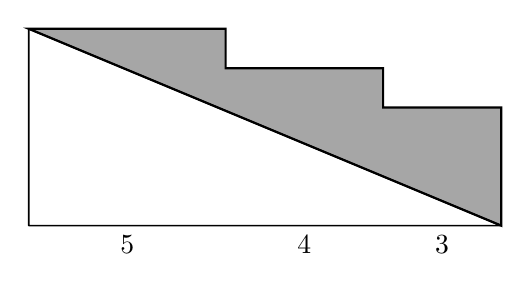
\begin{tikzpicture}[scale=0.50]
\tkzInit[xmin=-0.4, xmax=12.3, ymin=-0.4, ymax = 5.2]

\tkzDefPoint(0.0,5.0){a}
\tkzDefShiftPoint[a](270:5){b}
\tkzDefShiftPoint[b](0:12.0){h}
\tkzDefShiftPoint[b](0:5){c}
\tkzDefShiftPoint[c](90:5){d}

\tkzDefShiftPoint[c](0:4.0){e}
\tkzDefShiftPoint[e](90:4){f}
\tkzDefShiftPoint[f](180:4){g}

\tkzDefShiftPoint[e](0:3.0){h}
\tkzDefShiftPoint[h](90:3.0){i}
\tkzDefShiftPoint[i](180:3){j}

\tkzFillPolygon[draw,
                line width = 0.8pt,
                fill = black!35](a,h,i,j,f,g,d)

\tkzDrawPolygon[line width = 0.6pt](a,b,h)

\tkzDrawSquare(b,c)
\tkzDrawSquare(c,e)
\tkzDrawSquare(e,h)

\tkzLabelSegment[below](b,c){$5$}
\tkzLabelSegment[below](c,e){$4$}
\tkzLabelSegment[below](e,h){$3$}
\end{tikzpicture}
\end{minipage}
\hspace{2mm}
\begin{minipage}{50mm}
\vspace*{1mm}
Figura na rysunku obok składa się z 3 kwadratów o podanych długościach boków. Wyznacz pole
      zacieniowanego  obszaru. %\iteml $P = 20$
\end{minipage}

\hspace*{-9mm}
\begin{minipage}{64mm}
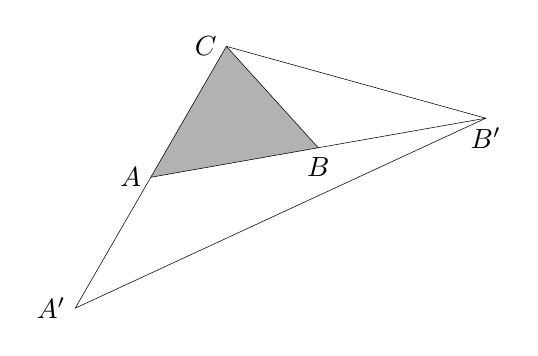
\begin{tikzpicture}[scale=1.0] % 57 mm
\tkzInit[xmin = -1.2, xmax=4, ymin = -1.5, ymax = 1.5]
%\tkzGrid
%\tkzClip
\tkzLength=1.2cm

\tkzDefPoint(0,0){A}
\tkzDefShiftPoint[A](10:1.8*\tkzLength){B}
\tkzDefShiftPoint[A](60:1.6*\tkzLength){C}
\tkzDefPointBy[homothety=center C ratio 2.0 ](A)    \tkzGetPoint{A'}
\tkzDefPointBy[homothety=center A ratio 2.0 ](B)    \tkzGetPoint{B'}

\tkzFillPolygon[fill = black!30](A,B,C)

\tkzDrawSegments(A,B B,C C,A B,B' C,B' A',B' A,A')
\tkzLabelPoints[left](A',A,C)
\tkzLabelPoints[below](B,B')
\end{tikzpicture}
\end{minipage}
\hspace{2mm}
\begin{minipage}{90mm}
% 61
Trójkąt $ABC$ na rysunku obok ma pole równe 7. Odcinek $AB'$ jest dwukrotnie dłuższy od odcinka $AB$,
      zaś odcinek $CA'$ jest dwukrotnie dłuższy od odcinka $CA$. Wyznacz pole trójkąta $AB'C$ oraz
      trójkąta $A'B'C$.
% \iteml $P_{AB'C}=14$, $P_{A'B'C}=28$
\end{minipage}


\vspace*{2mm}

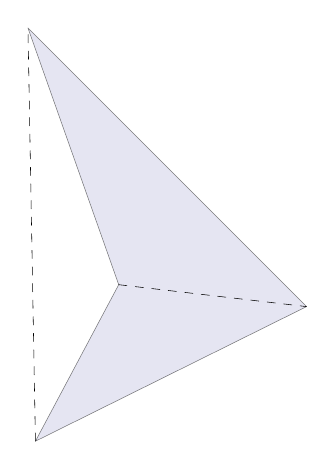
\begin{tikzpicture} [shift={(0,-9)},
rotate=-58,scale=1.5]
\tkzDefPoint(1.5,1.5){A}
\tkzDefPoint(2.25,0.2){B}
\tkzDefPoint(2.5,2.75){C}
\tkzDefPoint(-0.75,2){D}
\tkzDrawPolygon[fill=black!50!blue!20!,%
opacity=.5](A,B,C,D)
\tkzDrawSegments[style=dashed](A,C B,D)
\end{tikzpicture}
\hspace{10mm}
\begin{tikzpicture}[scale=.75]
\tkzDefPoint(0,0){A} \tkzDefPoint(8,0){B}
\tkzDefSquare(A,B) \tkzGetPoints{C}{D}
\tkzDrawPolygon(B,C,D,A)
\tkzClipPolygon(B,C,D,A)
\tkzDefPoint(4,8){F}
\tkzDefTriangle[equilateral](C,D)
\tkzGetPoint{I}
\tkzDrawPoint(I)
\tkzDefPointBy[projection=onto B--C](I)
\tkzGetPoint{J}
\tkzInterLL(D,B)(I,J) \tkzGetPoint{K}
\tkzDefPointBy[symmetry=center K](B)
\tkzGetPoint{M}
\tkzDrawCircle(M,I)
\tkzCalcLength(M,I) \tkzGetLength{dMI}
\tkzFillPolygon[color = orange](A,B,C,D)
\tkzFillCircle[R,color = yellow](M,\dMI pt)
\tkzFillCircle[R,color = blue!50!black](F,4 cm)%
\end{tikzpicture}


\begin{minipage}{60mm}
\begin{battleship}[rows=6, columns=6,scale=0.9, sbindent=10mm, sbwidth=5.5cm]
  \shipH{2,1,3,1,2,1}
  \shipV{1,2,1,3,2,1}
  \placesegment{3}{3}{\Fala}
  \placesegment{5}{4}{\ShipL}
  \shipbox{1,1,1,2,2,3}
\end{battleship}
\end{minipage}
\hspace{3mm}
\begin{minipage}{48mm}
\begin{kakuro}[rows=5,columns=4,color=yellow,scale=1.2]
\framepuzzle
\kakurorow{5}{\Black    ,\KKR{12}{} ,\KKR{19}{} ,\Black     }
\kakurorow{4}{\KKR{ }{4},      3    ,     1     ,\KKR{7}{}  }
\kakurorow{3}{\KKR{}{21},      8    ,     9     ,     4     }
\kakurorow{2}{\KKR{ }{9},      1    ,     6     ,     2     }
\kakurorow{1}{\Black    ,\KKR{ }{4} ,     3     ,     1     }
\end{kakuro}
\end{minipage}
\hspace{1mm}
\begin{minipage}{60mm}
\begin{battleship}[rows=6, columns=6,scale=0.9, sbindent=10mm, sbwidth=5.5cm]
  \shipH{2,2,0,3,1,2}
  \shipV{1,2,3,1,1,2}
  \placesegment{4}{1}{\Fala}
  \placesegment{1}{2}{\ShipB}
  \shipbox{1,1,1,2,2,3}
\end{battleship}
\end{minipage}\\[5mm]


Rozwiąż poniższe dwa algebrafy:\\[2mm]
\hspace*{10mm}
\begin{minipage}{51mm}
\LARGE
\begin{verbatim}
 AB + AB = CBB
  +    +     +
CAB + CA = CDA
\end{verbatim}
\hrule\vspace{-2mm}
\begin{verbatim}
EBB + DA = EDA
\end{verbatim}
\end{minipage}
\hspace{15mm}
\begin{minipage}{52mm}
\LARGE
\begin{verbatim}
AAB -  B = AAC
  -    +     -
 BB + DB = ACC
\end{verbatim}
\hrule\vspace{-2mm}
\begin{verbatim}
 EC - BC =  AC
\end{verbatim}
\end{minipage}




\hspace*{-1mm}
\begin{minipage}{97mm}
  \begin{lpsudoku}
  \setrow{9}{{ },{2},{ },{8},{ },{1},{ },{6},{ }}
  \setrow{8}{{7},{ },{ },{ },{2},{ },{ },{ },{3}}
  \setrow{7}{{ },{1},{ },{7},{ },{6},{ },{4},{ }}
  \setrow{6}{{2},{ },{6},{ },{ },{ },{8},{ },{1}}
  \setrow{5}{{3},{ },{ },{ },{ },{ },{ },{ },{5}}
  \setrow{4}{{5},{ },{8},{ },{ },{ },{6},{ },{7}}
  \setrow{3}{{ },{8},{ },{1},{ },{3},{ },{5},{ }}
  \setrow{2}{{9},{ },{ },{ },{5},{ },{ },{ },{8}}
  \setrow{1}{{ },{5},{ },{9},{ },{2},{ },{7},{ }}
\end{lpsudoku}
\end{minipage}
\hspace{2mm}
\begin{minipage}{68mm}
Wypełnij diagram sudoku.
\vspace*{2mm}
 Jackowi zabrakło 7 złotych na kupno książki, a Bogdanowi 2 złotych. Jednak gdy oni zebrali razem
      swoje pieniądze, to nie starczyło ich nawet na zakup jednej książki.  Każdy z nich miał przynajmniej
       1\,zł. Ile kosztowała książka, jeżeli    wiadomo, że była to całkowita liczba złotówek?
\vspace{2mm}
Do liczby 10 dopisz z obu stron po jednej cyfrze, tak aby otrzymał liczbę  podzielną przez 36.
\vspace{2mm}
Ile liczb dwucyfrowych o niejednakowych cyfrach można utworzyć z  cyfr 0, 1, 2, 3, 4, 5, 6?
\end{minipage}\\[3mm]

% 4
 Wpisz brakujące cyfry w  arytmografach:\\
\begin{minipage}{65mm}
 \Large
 \begin{tabular}{ccccccc}
        &        & \Ramka & \Ramka & \Ramka & \Ramka  \\       %   ####
        &        &    *   &        & \Ramka &    2    \\       %   * #2
 \cline{2-6}                                          \\[-6mm] % ______
        &    1   &    8   & \Ramka &    4   &    8    \\       %  18#48
    7   &    4   &    9   &    9   & \Ramka           \\       % 7499#
 \cline{1-6}                                          \\[-6mm] % ______
 \Ramka & \Ramka & \Ramka &    6   &    6   & \Ramka           % ###66#
 \end{tabular}
\end{minipage}
\hspace{10mm}
\begin{minipage}{65mm}
 \Large
 \begin{tabular}{ccccccc}
        &        &    3   &    3   &    4     \\                 %  334
        &    *   & \Ramka & \Ramka & \Ramka   \\                 % *###
 \cline{2-5}                                  \\[-6mm]           %  ___
        &        & \Ramka & \Ramka &    8     \\                 %  ##8
    1   & \Ramka & \Ramka &    2              \\                 %1##2
 \Ramka & \Ramka & \Ramka                     \\                 %###
 \cline{1-5}                                  \\[-6mm]           %_____
    4   & \Ramka & \Ramka & \Ramka & \Ramka                      %4####
 \end{tabular}
\end{minipage}



 Za czwartym  razem  Porcja w jednej ze szkatułek umieściła portret, a na szkatułkach umieściła
      następujące napisy:


\hspace*{10mm} ZŁOTA \hspace{43mm} SREBRNA \hspace{38mm} OŁOWIANA\\[2mm]
\hspace*{1mm}
\fbox
{
\begin{minipage}{35mm}
1)\,Portretu nie ma w tej szkatułce.\\
2)\,Twórca portretu pochodzi z Wenecji.
\end{minipage}
}
\hspace{16mm}
\fbox
{
\begin{minipage}{38mm}
1)\,Portretu nie ma w złotej szkatułce.\\
2)\,Twórca portretu pochodzi z Florencji.
\end{minipage}
}
\hspace{16mm}
\fbox
{
\begin{minipage}{35mm}
1)\,Portretu nie ma w tej szkatułce.\\
2)\,Portret jest w srebrnej szkatułce.
\end{minipage}
}

\vspace*{3mm}

  Porcja wyjaśniła zalotnikom, że na żadnym wieku nie ma więcej niż jednego fałszywego zdania.
  W której wobec tego szkatułce znajduje  się  jej portret?

\noindent
\begin{minipage}{55mm}
Wykres funkcji $f$ składa się z 9 punktów i wygląda tak jak na  rysunku obok.\\
Linią ciągłą narysowany jest wykres funkcji, również określonej wzorem $y = \frac 12 x^2 + 1$, której dziedziną
jest zbiór wszystkich liczb z przedziału $[-4,4]$.
\end{minipage}
\hspace*{5mm}
\begin{minipage}{70mm}
    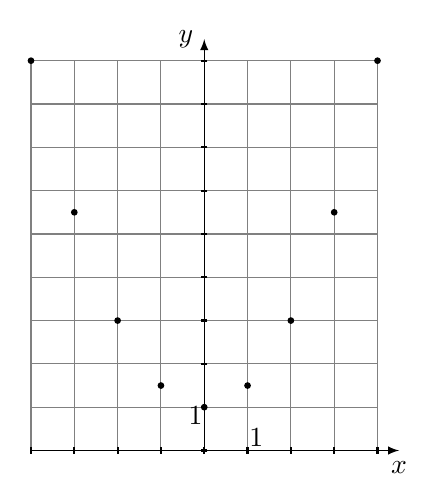
\begin{tikzpicture}[scale=0.55]
    \tkzInit[ xmin = -4,
    xmax =  4,
    ymin =  0,
    ymax =  9
    ]
    \tkzGrid
    \tkzDrawXY
    \tkzDefPoint(-4,9){A}
    \tkzDefPoint(-3,5.5){B}
    \tkzDefPoint(-2,3){C}
    \tkzDefPoint(-1,1.5){D}
    \tkzDefPoint(0,1){E}
    \tkzDefPoint(1,1.5){F}
    \tkzDefPoint(2,3){G}
    \tkzDefPoint(3,5.5){H}
    \tkzDefPoint(4,9){I}
    \tkzDrawPoints(A,B,C,D,E,F,G,H,I)
    \tkzFct[domain = -4:4]{0.5*x*x + 1}
    \node at ( 1.2, 0.3) {1};
    \node at ( -0.2, 0.8) {1};
    %\node at (-4, 4.4) {funkcja $f$};
    \end{tikzpicture}
\end{minipage}

\end{document} 